\graphicspath{{../images/ch3/}}	% Image directory


\chapter{Experimental study of ion conductance property of hybrid conductor-insulator nanopores}

	

	\section{Background}
	
		In the introduction of this thesis we discussed the electrical double layer (EDL) which is a screening layer of ions that forms in the proximity of a charged surface. The vast majority of pores studied are non-conductive insulators, and their surface charge properties come from the functionalization of chemical groups at their surface. For instance, the base of the pore studied in this section is $\mathrm{Si{3}N_{4}}$ (silicon nitride), whose native silane chemistry means there are exposed alcohols at the surface that are either negative or neutral depending on pH. However, charge on a surface can arise \textit{via} other means. When a metal is exposed to an electric field, electrons in the metal rapidly redistribute themselves on the surface to cancel the external applied field. If we assume the metal was originally overall neutral, the charge pattern will consist of an abundance of negatively-charged electrons at one end and an abundance of positively-charged holes at the other. A natural question is whether these \textit{induced} charges have associated EDLs in the same way that static charges do.
		
		Previous studies suggest they do. For instance, Squires \textit{et al.} and Pascall \textit{et al.} performed experiments with applied external electric fields on various metal surfaces and discovered that electroosmotic flow occurred. They reasoned that electroosmosis was a result of polarization of charges according to the model discussed above \cite{Squires2004, Pascall2010}. However, these types of induced-charges have been seldom discussed in hte context of nanopore transport, especially in the context of an realizable experimental platform. In order to understand the effect of induced charges on nanopore transport, we considered a hybrid metal-insulator pore created by evaporating a thin layer of gold onto the pore surface. If the pore was only the insulator, its IV curve would be symmetrical due to the lack of any symmetry breaking in the system. The addition of the metallic layer breaks this symmetry, and we expect to see ionic current rectification in the pore (see chapter 1.) However, ionic current rectification alone is insufficient for proving that induced surface charges contribute to the pore's conductance; this is because essentially \textit{any} symmetry breaking in a pore, including a difference in static surface charges between two regions, a difference in geometrical shape between two regions, \textit{or} induced surface charges, will lead to ionic current rectification.
		
		\begin{figure}
			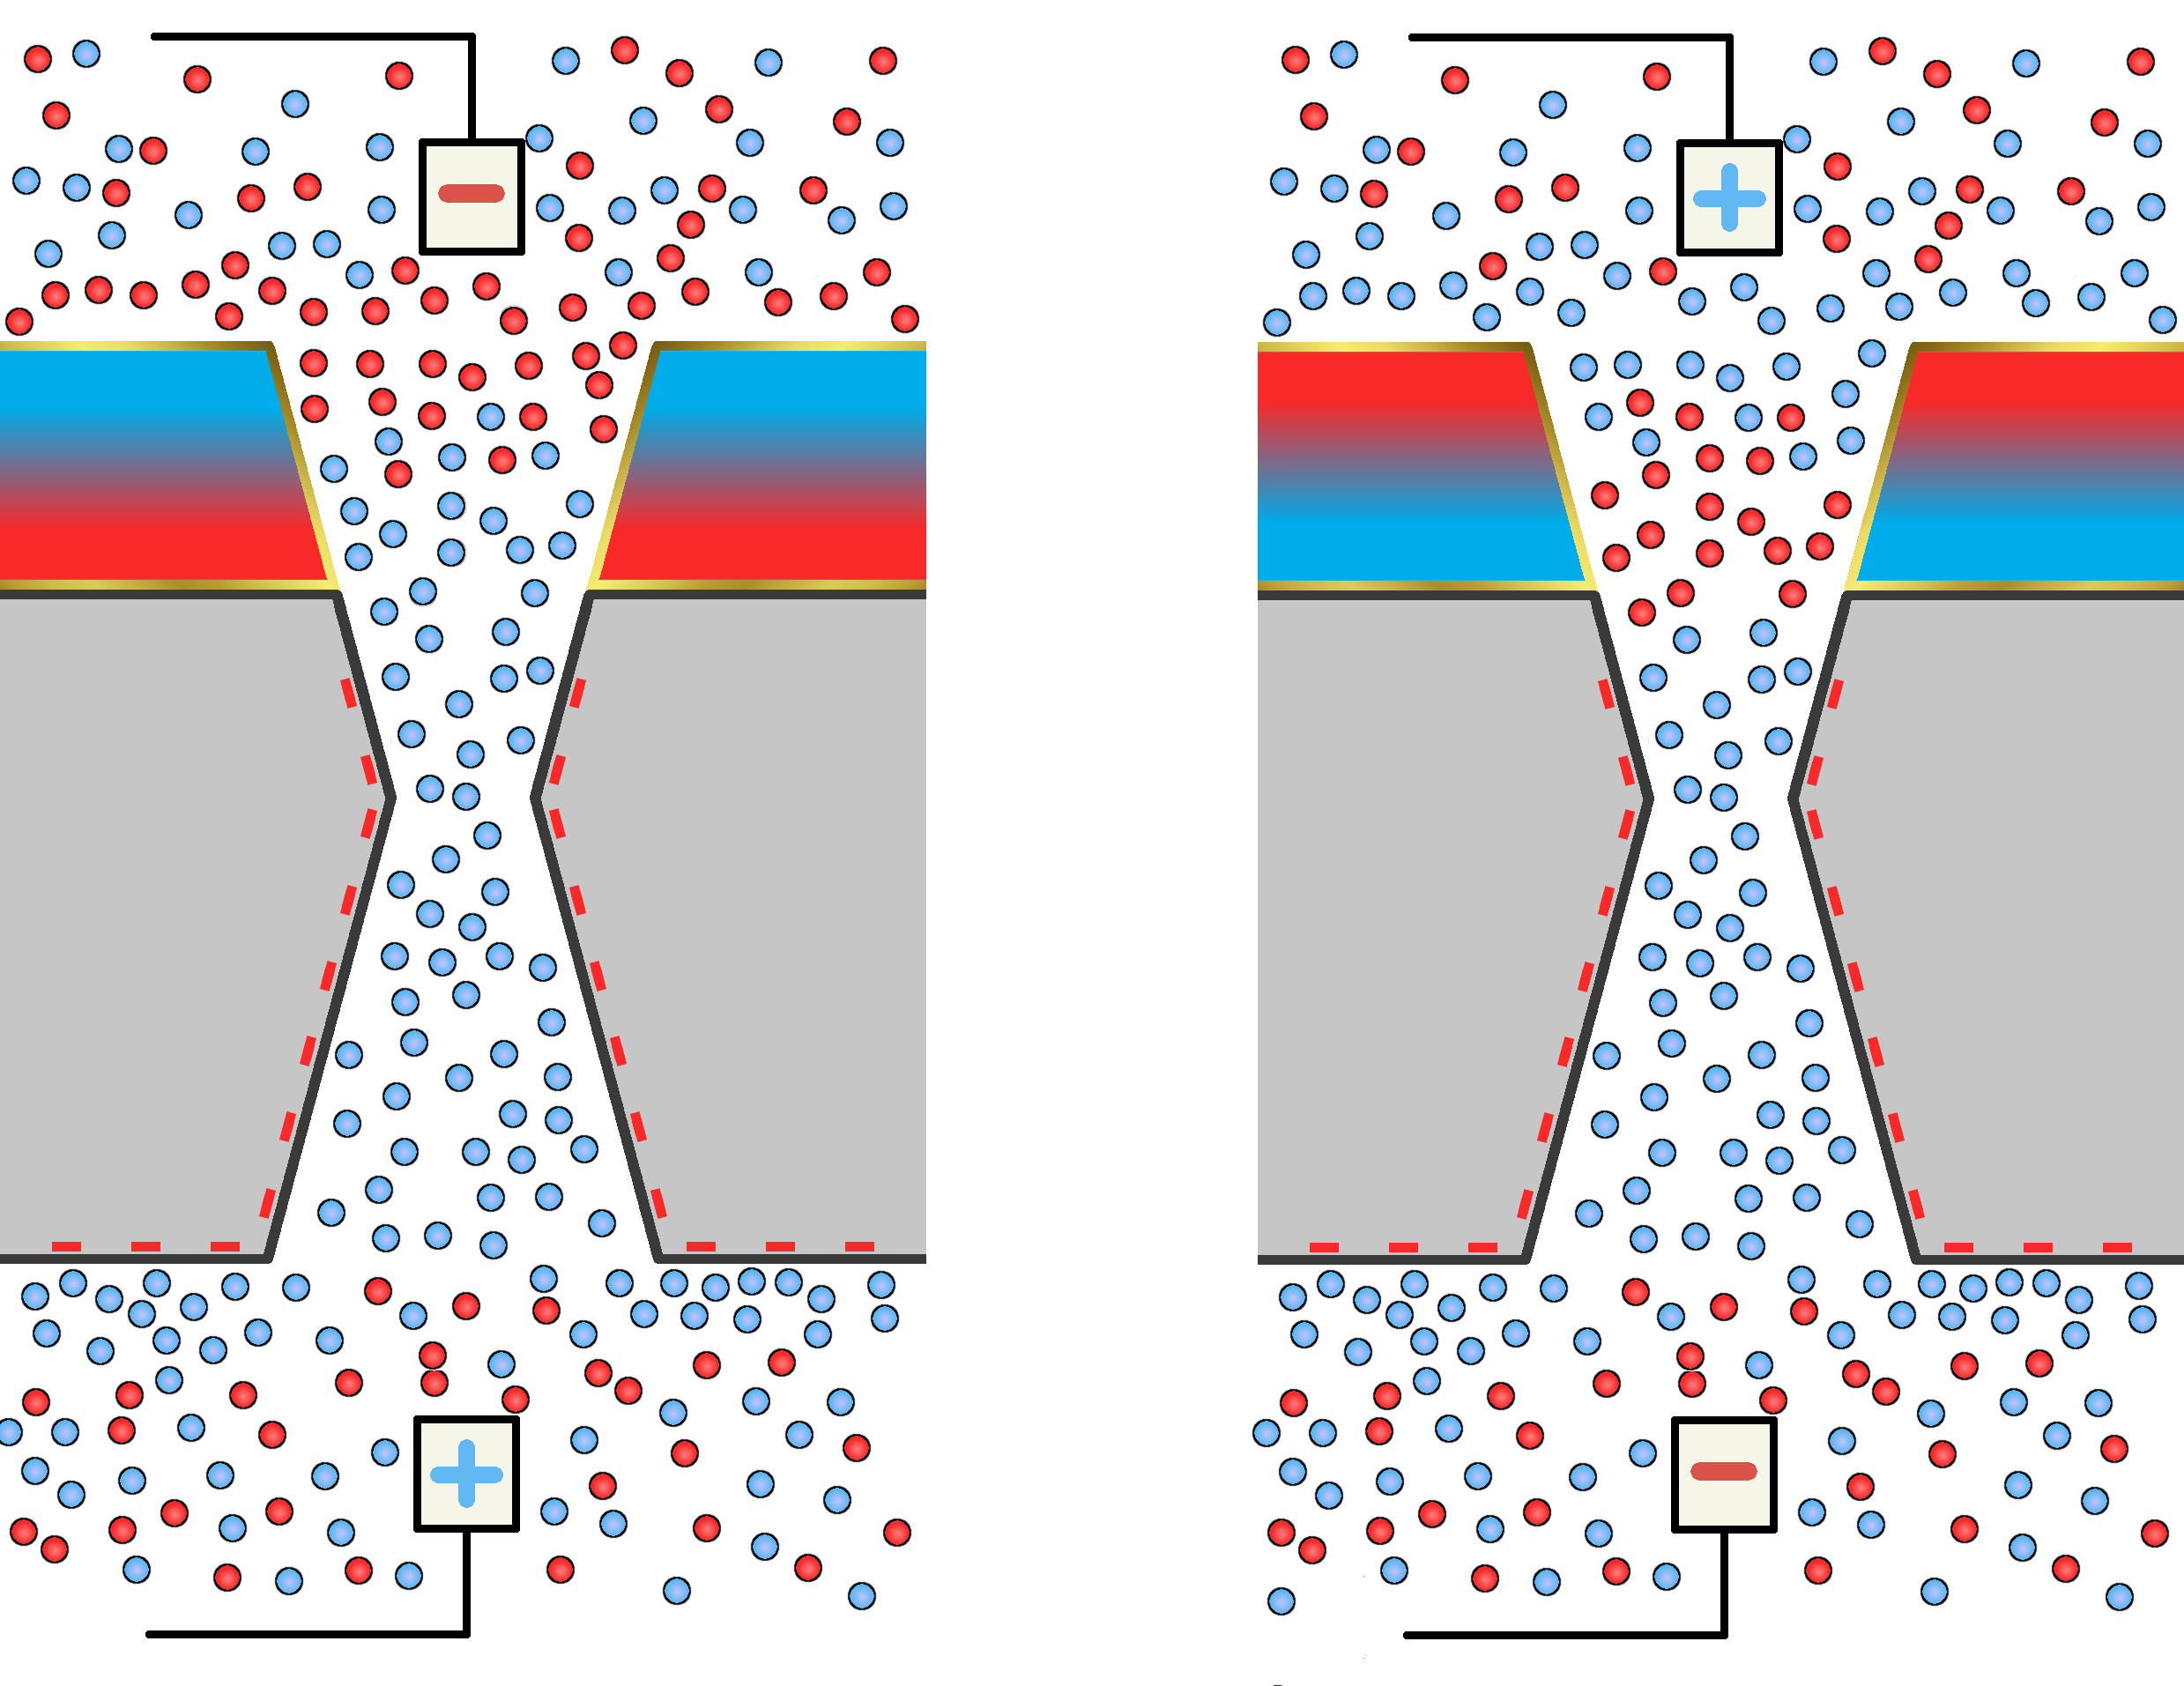
\includegraphics[width=0.5\textwidth]{SiN-Gold_Model.png}
			\caption{\textbf{Model for the induced-charge and EDL charges in the hybrid conductor-insulator nanopore.} \textbf{Left:} Negative bias applied to gold side. \textbf{Right:} Positive bias applied to gold side. For the positive bias, a depletion zone forms at the junction between the gold and SiN, which is expected to severely limit the conductance. For the negative bias, no depletion zone forms and therefore the conductance is expected to be unhindered. The double conical geometry reflects the expected geometry of SiN pores drilled \textit{via} a transmission electron microscope electron beam.}
			\label{fig:SiNGoldModel}
		\end{figure}

		
		In order to provide evidence that induced charges directly contributed to a pore's conductance properties in this system, we need to devise a model for the manner of the induced rectification properties, and to check if the model accurately describes experimental data. Figure \ref{fig:SiNGoldModel} is a scheme of the induced-charge model, which is effectively explained by the surface charges present. First, the insulating part of the pore has an approximately uniform surface charge due to ionization of the chemical groups on its surface. On the gold, the charge patterning depends on the applied voltage. When a negative bias is applied on the gold side of the pore, electrons are repelled from the electrode while holes are attracted. The charge pattern in the solution from top to bottom is then $-++$. On the other hand, when a positive bias is applied on the gold-side of the pore, holes flee to the inside of the pore while electrons are drawn towards the electron. Therefore, from the positive electrode to the negative electrode the surface charge pattern is $+-+$ (right hand side of figure \ref{fig:SiNGoldModel}. The primary difference in the charge pattern as it relates to the influence on the nanopore between the two voltage polarity cases is the charge juntion at the conductor-insulator interface; in the latter case (positive voltage applied on the metallic side), the $+-$ junction indicates the presence of a bipolar junction that leads to a depletion zone in the EDL, as discussed in the section on ionic current rectification in chapter 1. This depletion zone is characterized by having a very large resistance, and therefore limits the total current through the pore. For the opposite polarity, the depletion zone is not present and therefore we do not expect any significant limiting of the current.
		
		This model, known as the induced-charge model for hybrid conductor-insulator nanopores, was tested experimentally in this work.
		
	\section{Experimental setup}
		
		In order to test the induced-charge model, we devised a platform consisting of thin nanopores in silicon nitride (SiN) with gold (Au) deposited on top. The crucial elements of this setup consisted of the silicon nitride (SiN) membrane, evaporated gold (Au) layer, transmission electron microscope drilling of the pore, and the current-voltage characterization measurements.
		
		\subsection{Silicon nitride}
			
			Silicon nitride was used as the substrate through which to drill the nanopore. The effects of polarization of the gold should be apparent in truly nano-scale systems, so it was important to choose a material through which a small pore could be fabricated. As of the writing of this thesis, silicon nitride (chemical formula $\mathrm{Si_{3}N_{4}}$) is a popular choice for creating small nanopores given its mechanical stability and well-understood surface chemistry. The method of pore formation, TEM drilling (discussed below) can enable pores ranging from $1-20$ nm in diameter, and is capable of drilling through substrate lengths of up to $100$ nm. It is predicted that pores with very low aspect ratios, i.e.~short pores, will have severely diminished rectification propeties. In order to ensure large rectification, the solution must be subjected to a sufficient length of EDL. In order to strike a compromise between TEM's capabilities and the undesirable low-aspect ratio effects, a substrate thickness of $\SI{50}{nm}$ was chosen. The silicon nitride substrate is commonly used in TEM microscopy, and therefore is available from commercial vendors. The substates were ordered from the SPI company. The substrate itself is grown onto a thicker layer of silicon, through which a window is drilled on the backside to expose the silicon nitride. The final result is a $\SI{50}{nm}$ thick layer of SiN supported by a silicon chip. After pore fabrication, silanol groups native to the pore surface act as surface charges if immersed in solution with pH beyond their pKa value of 
			
		\subsection{Gold deposition}
			
			Although the model of induced-charge rectification described above is independent of the type of conductor used, we chose to use gold (Au) because of its mechanical stability after deposition and its resistance to corrosion and oxidation, which could create a surface chemistry effect that could potentially obscure the relationship with the induced surface charges. With the conductor's material chosen, we think about the desired deposition thickness. In the model of induced-charge rectification described above, it is necessary to have a bipolar junction far enough inside the pore that a depletion layer can form. For this reason, we aimed to deposit a $\SI{30}{nm}$ layer of gold onto the surface of the SiN. There are a number of means of depositing metals onto surfaces, but given the thinness of the desired layer we chose to deposit \textit{via} an e-beam evaporation. During e-beam evaporation, a chunk of metal is pumped down in vaccuum and bombarded with high-energy electrons. The combination of low-pressure and large temperature caused by the bombardment with the electrons causes individual metal atoms to evaporate from the surface of the chunk along straight-line or ray paths. The atoms then hit the surface of the substrate, which is suspended above it, and stick. Although Au \textit{can} be deposited directly onto the surface of SiN, a thin layer ($\SI{3}{nm}$) of chromium (Cr) was first evaporated, which facilitates adhesion of the Au.
			
		\subsection{Transmission electron microscope drilling}
		
			\begin{figure}
				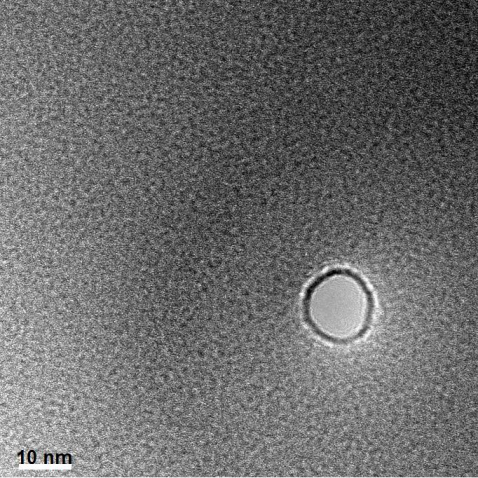
\includegraphics[width=0.5\textwidth]{sinpore.png}
				\caption{\textbf{A $\sim\SI{15}{nm}$ SiN pore drilled \textit{via} TEM.}}
				\label{fig:sinpore}
			\end{figure}

		
			The transmission electron microscope (TEM) is a super resolution imaging technique that is typically used to image objects below the optical diffraction limit of $\SI{200}{nm}$. However, if the electron beam is sufficiently energized and focused, the electron beam can act as a drill for forming nanopores instead of for imaging. This technique was used to drill pores through the SiN-Au hybrid device described in the above two steps. A highly focused beam in the TEM's scanning (S) mode is applied to the surface. The energetic electrons strike the surface and eject atoms, while simultaneously the entire structure melts. The final result is a pore with the same thickness as the substrate, and with a double conical geometry which is a result of the simultaneous ballastic ejection and melting. Because the drilling is performed inside the TEM, the resulting pore can also be immediately imaged. Figure \ref{fig:sinpore} shows an example of a $\sim\SI{15}{nm}$ TEM-drilled pore.
			
		\subsection{Pore conductance characterization}
		
			\begin{figure}
				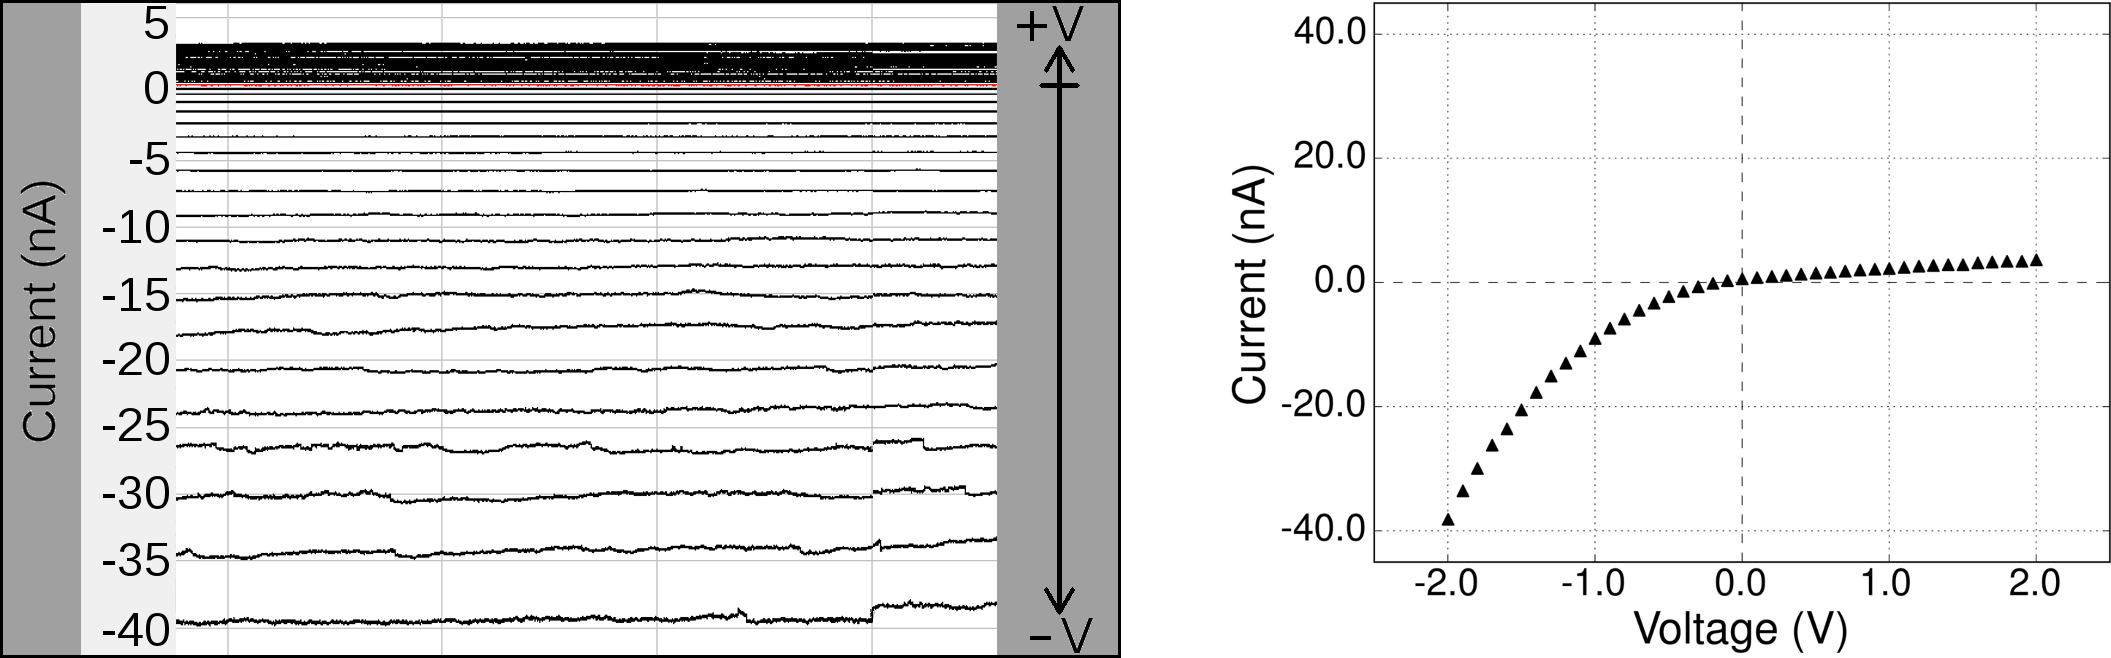
\includegraphics[width=\textwidth]{siniv.png}
				\caption{\textbf{A current-voltage time series alongside the current-voltage curve produced from it.} \textbf{Left}: Current-voltage time series. Each continuous line corresponds to one voltage setting; once a voltage value is set, the current does not significantly vary. \textbf{Right}: Traditional pore I-V curve. The asymmetry in the current with respect to voltage (present in both signals) is the hallmark indicator of ionic current rectification.}
				\label{fig:siniv}
			\end{figure}

		
			In order to test the induced-charge model, we measured the current-voltage (IV) response of each of the fabricated nanopores in $100$ and $500$ mM KF and KCl salt solutions. The total surface charge of a pore `felt' by the ions in the solution is given by a combination of the ionized chemical groups on its surface and any chemical species that are adsorbed to the surface. Cl is known to adsorb to the surface of gold, and so we expect that the gold in KCl solutions will have net charge given by the adsorbed chloride ions and the induced-charges. For this reason, measurements were performed primarily with KF solution. However, it was predicted that adsorption of chloride on the Au surface would diminish the effects of the induced-charge, and this model was tested by performing measurements with KCl on chips that had already been measured in KF, to see if their conductance behavior changed according to this prescription. 
			
			Due to the small sizes of the pore and the low surface charge density of the silanols on the SiN surface, the interior of the pore is difficult to wet, meaning any vapor present inside the pore can be stable and difficult to remove. If this is the case, ions cannot pass through. Often times these vapor phases are quasi-stableand the pore will spontaneously wet and dewet. In order to reduce these hydrophobic effects, we use an even 50/50 mixture of water and ethanol solvent; the combination of both solvents promotes wetting of the pore. 
			
			In principle, during IV measurements one needs only to sweep the voltage along the desired range, stopping to record the current at each voltage value. Usually one delays $\sim\SI{1}{second}$ after changing the voltage before a current measurement is made to allow for the system to equilibrate, e.g.~due to system capacitance charging/discharging. However, in systems in which the system conductance can stochastically change, e.g.~due to spontaneous wetting/dewetting transitions, it is advantageous to record a time series of the current voltage sweeps rather than measure single data points. If a transition occurs, it can be observed in the time series of the signal and appropriately dealt with afterwards. The protocol for measuring IV curves is then to apply a fixed voltage, record the current for a fixed amount of time, and repeat for all of the desired voltages. Then, an IV curve is produced by averaging the current time-series for a fixed interval of time (averaging is performed to smooth over the small amount of noise in the signal). In this study, voltages were applied for a total of $\SI{20}{s}$ and the current values in the last $\SI{0.5}{s}$ were averaged to create the current measurement value. Figure \ref{fig:siniv} shows an example current-voltage time series and the IV curve produced from it for one of the pores used in the study measured in KF solution. On the left is a current-voltage time series plot that shows the current value time series for different voltage settings, while the right hand side of the figure shows a traditional I-V curve of the pore.  
			
			
	\section{Experimental results}
	
		A number of conductor-insulator pores were tested, along with plain SiN pores to test of the pores intrinsically rectify the current (e.g.~due to a geometrical asymmetry).
		
		\begin{figure}
			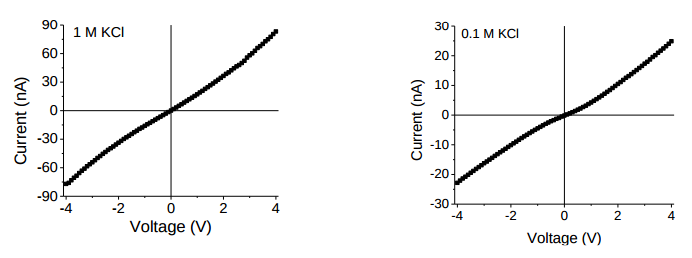
\includegraphics[width=\textwidth]{sinsymm}
			\caption{\textbf{IV curves taken of bare SiN pores}. The symmetry in the IV curve reveals no inherent rectification of the TEM drilled pores.}
			\label{fig:sinsymm}
		\end{figure}
		
		\begin{figure}
			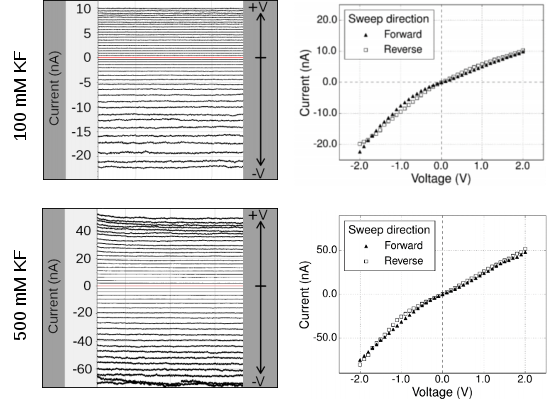
\includegraphics[width=\textwidth]{sinau0}
			\caption{\textbf{IV curves taken of Au-SiN pore in $\SI{100}{mM}$ and $\SI{500}{mM}$ KF.} The symmetry in the IV curve reveals no inherent rectification of the TEM drilled pores. The ion rectification ratio $R$ is lower in the higher concentration solution, as is expected from basic considerations of EDL thickness.}
			\label{fig:sinau0}
		\end{figure}
		
		\begin{figure}
			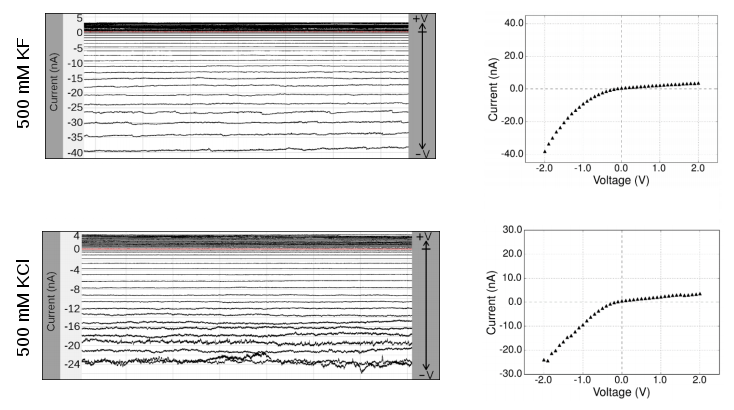
\includegraphics[width=\textwidth]{sinau1}
			\caption{\textbf{IV curves taken of Au-SiN pore in $\SI{500}{mM}$ KCl and KF.} The rectification ratio $R$ is lower in the KCl solution than in the KF solution, which is expected due to the additional contribution of the static charge from adsorbed $\mathrm{Cl^{-}}$ ions on the gold surface.}
			\label{fig:sinau1}
		\end{figure}


		
		Figure \ref{fig:sinsymm} shows two IV curves gathered for the SiN-only (insulator pore only). The plot shows approximately symmetric IV curves, indicating a symmetric nanopore. 
		
		On the other hand, figure \ref{fig:sinau0} shows two IV curves collected for a single nanopore approximately $\SI{9}{nm}$ in diameter. The IV curves taken in KF show significant rectification, with a ratio of approximately $R=0.5$ for the $\SI{100}{mM}$ concentration and $R=0.7$ for the $\SI{500}{mM}$ KF concentration. The increase in rectification $R$ towards $R=1$ with increasing salt concentration is consistent with the decrease in thickness of the EDL. In the model we developed for the induced-charge rectification, a depletion region is expected to form in the interior of the pore. Typically pores that have depletion zones experience much greater rectifications due to the `off-state' voltage polarity having nearly zero conductance. While this pore's rectification is not small enough (e.g.~not close to zero) to describe it as an ionic diode, the rectification direction is nevertheless consistent with the proposed model. We note that this direction of rectification is inconsistent with models having only static charges on the SiN and Au, barring the case where the $Au$ has positive charges adsorbed onto its surface, which is unexpected for the ion species used in this study.
		
		In order to understand the effect of a static charge superimposed on top of the induced-charge, we next performed experiments in KCl in addition to KF. Figure \ref{fig:sinau1} shows a $\SI{12}{nm}$ pore with IV curves measured in $\SI{500}{mM}$ concentration of both types of salts. Note that both salts give the same type of rectification as in the previous example. This result is not entirely unexpected, as the presence of adsorbed chloride will bring the two charges in the depletion zone closer together in magnitude, while still maintaining a finite, albeit reduced rectification. If the $Cl^{-}$ ions adsorbed to the surface of the gold to the extent that they dominated both the induced-charge on the gold and the surface charge on the SiN, then it is possible the rectification direction could even flip direction such that $R>1$. However, we did not observe such an effect.
		
	\section{Modelling results}
		
		In order to provide an additional line of evidence pointing to induced-charge based ion current rectification found in experiments, we performed finite-element analysis simulations using the COMSOL Multiphysics software package. The models were designed to emulate the experimental set up, e.g.~the channel geometries and salt concentrations used were similar. However, rather than try to reproduce the double conical geometry expected for TEM drilled pores, we worked with a cylindrical geometry which greatly facilitated convergence of the solutions with the very minor penalty of not adhering exactly to the experimental conditions. Because the cone angle is expected to be shallow and because the COMSOL results are meant to be interpreted semi-quantitatively, and are primarily used to draw conclusions about the rectification direction and mechanism, replicating the exact geometry of the pore was deemed unneccessary. Details of the COMSOL simulation can be found in the appendix.
		
		\begin{figure}
			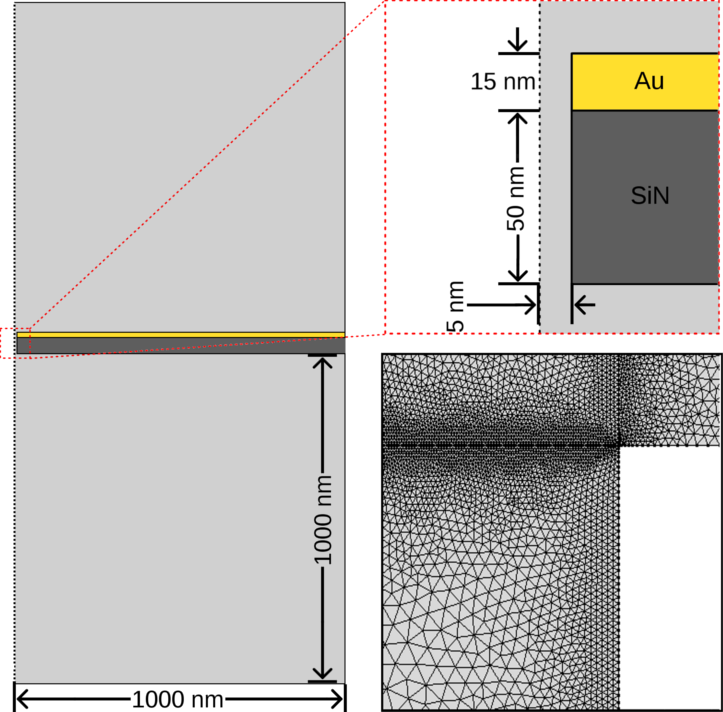
\includegraphics[width=\textwidth]{comsol_model}
			\caption{\textbf{COMSOL simulations.}}
			\label{fig:comsolmodel}
		\end{figure}
		
		\begin{figure}
			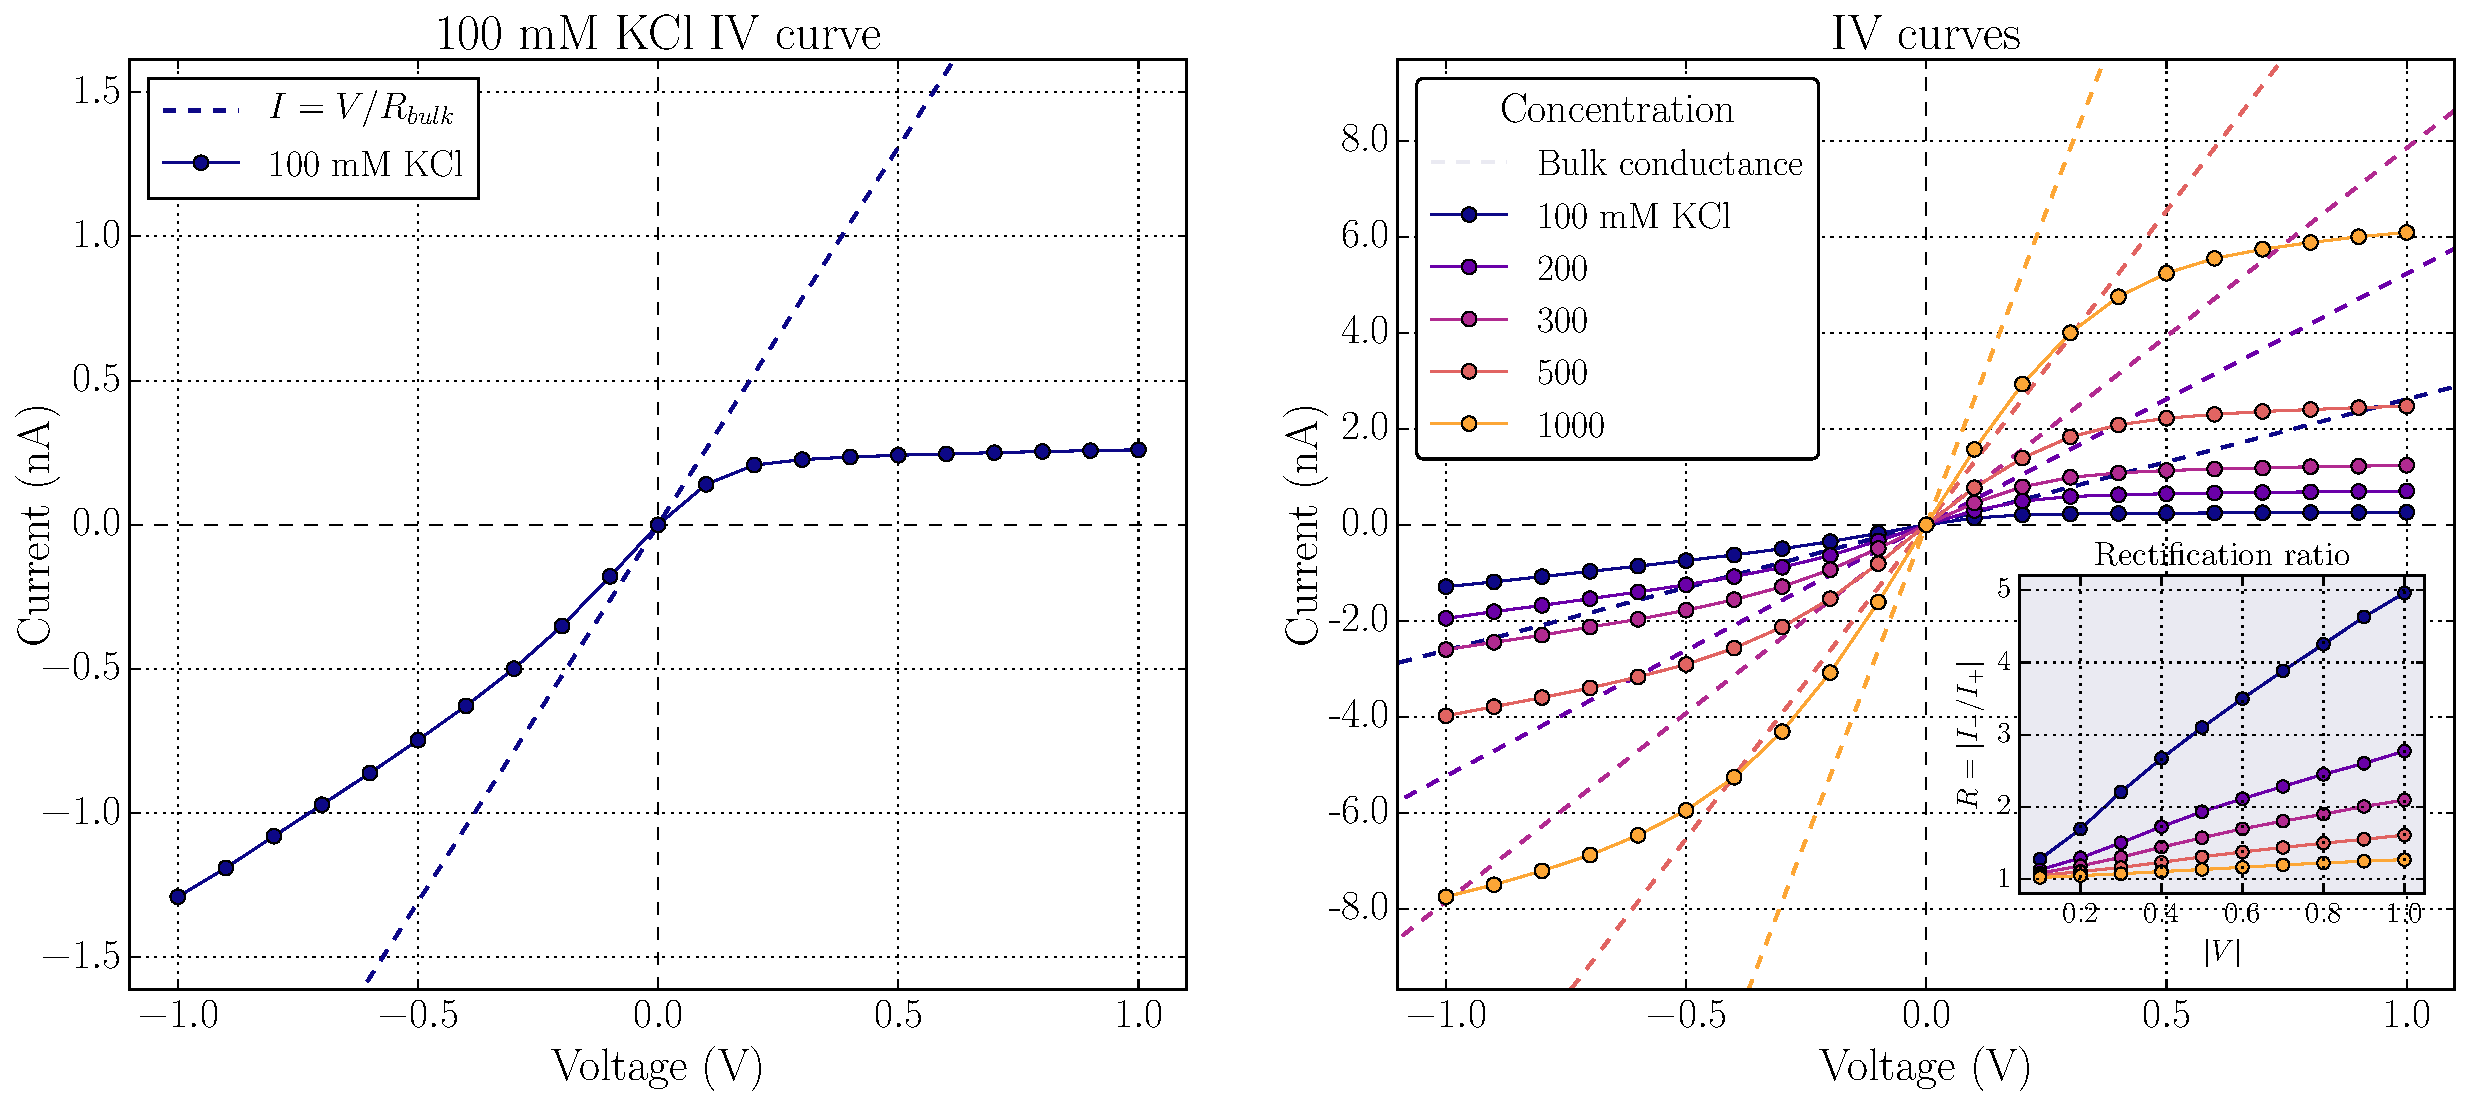
\includegraphics[width=\textwidth]{comsol1}
			\caption{\textbf{COMSOL simulations.}}
			\label{fig:comsol1}
		\end{figure}
		
		\begin{figure}
			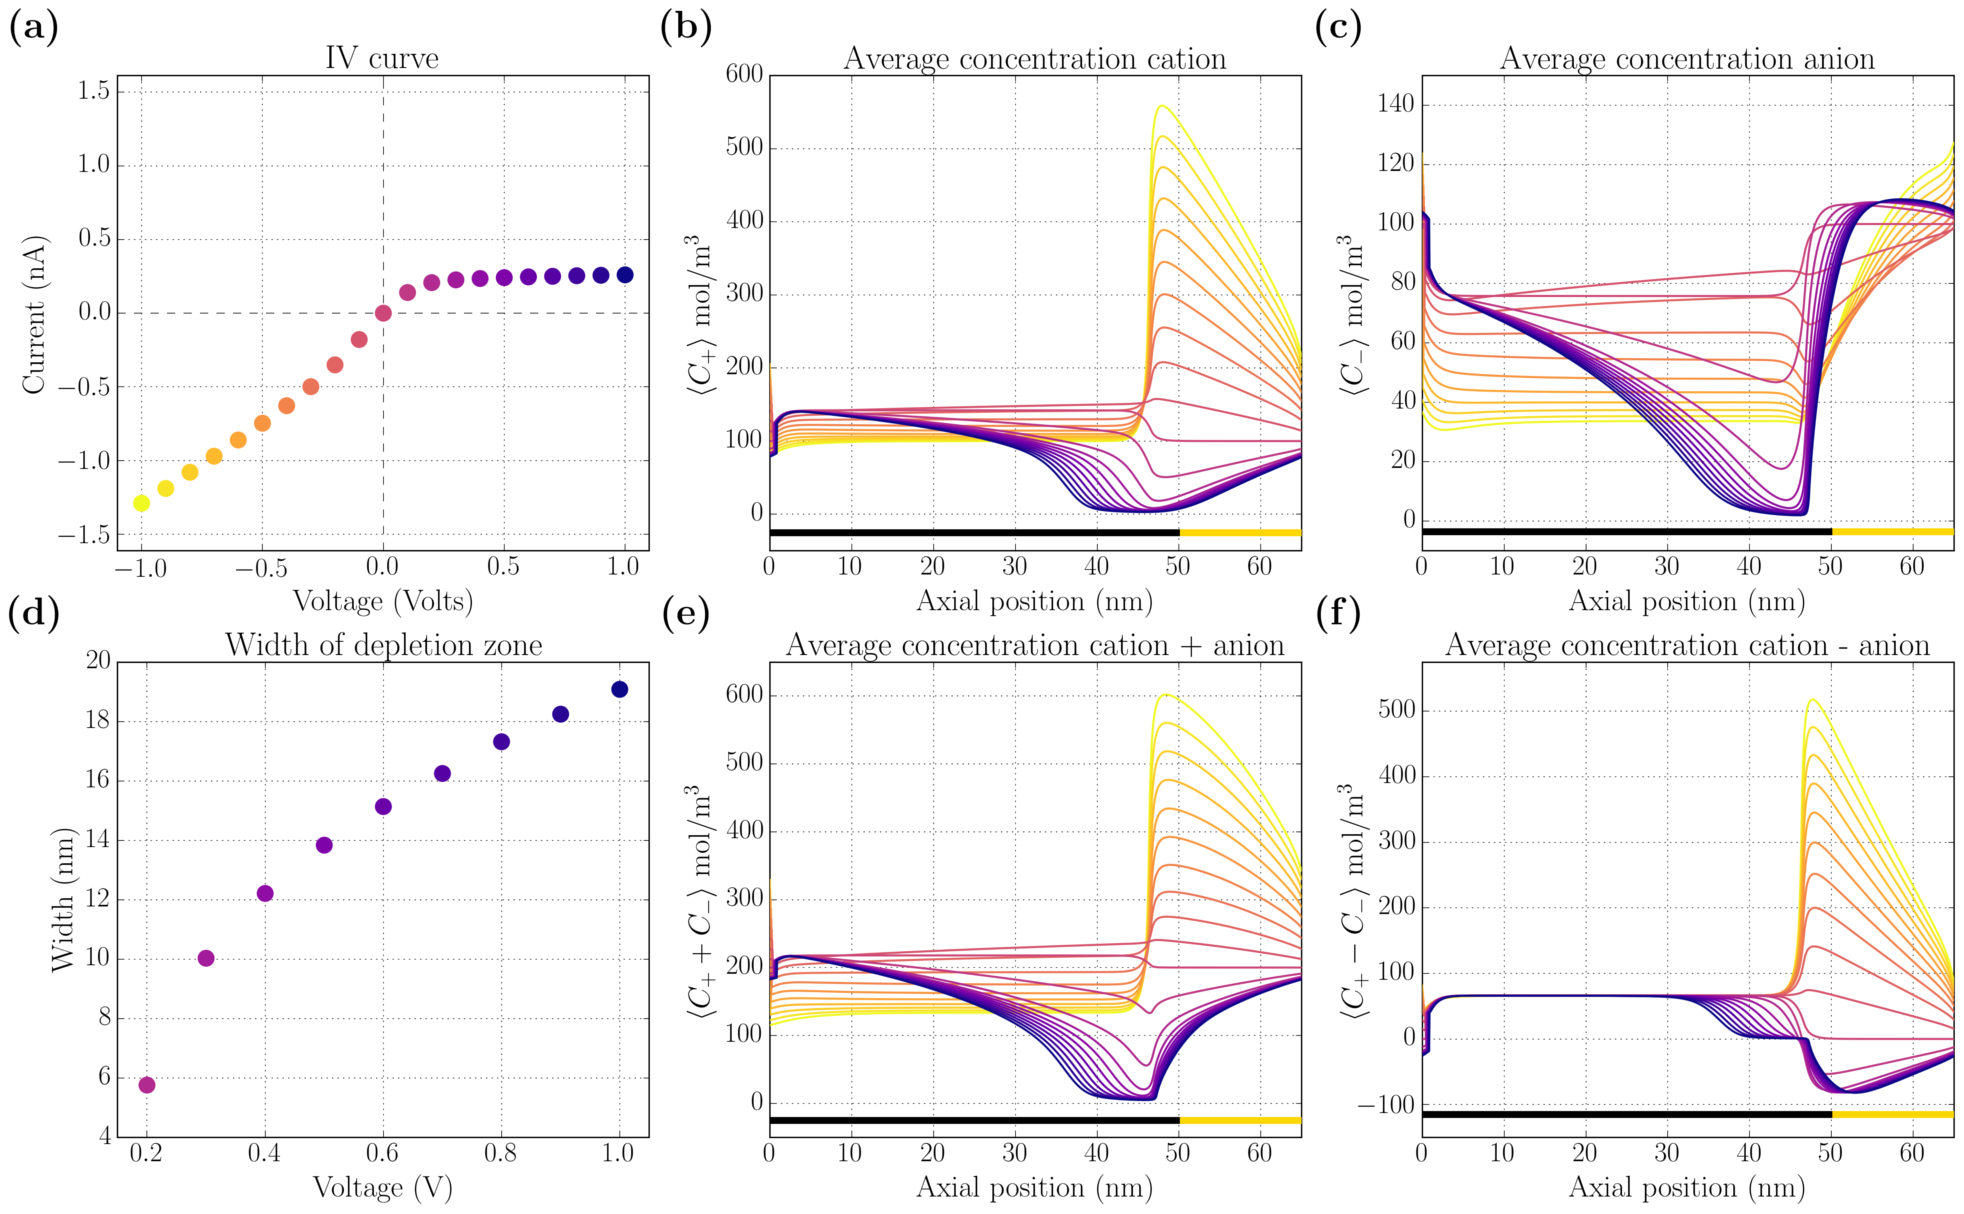
\includegraphics[width=\textwidth]{comsol2}
			\caption{\textbf{COMSOL simulations.}}
			\label{fig:comsol2}
		\end{figure}
		
		The results of the simulations are found in figures \ref{fig:comsol1} and \ref{fig:comsol2}. We simulated IV curves for the model device and calculated the average concentrations of the cations, anions, and combinations at various axial positions inside the pore, and used these calculations to calculate the width of the depletion zone that forms for positive voltages. Figure \ref{fig:comsol1} shows IV curves of the simulated pore at various concentrations. Notice htat at low concentrations the pore rectifies in the negative direction i.e. $R=|I_{-}/I_{+}|>1$ and the rectification ratio $R$ decreases with increasing electrolyte concentration, both results are consistent with the experimental data. Figure \ref{fig:comsol2} shows the average concentrations of $C_{K}$, $C_{Cl}$, $C_K+C_Cl$ and $C_K-C_Cl$ at various axial positions. The concentrations of $C_{K}$ and $C_{Cl}$ along the length of the gold surface are consistent with the polarization model of gold: when a positive potential is applied on the side of the metal, electrons are drawn to the entrance of the pore, inducing formation of an EDL more positive than at the opposite terminal, and the opposite occurs for the opposite voltage. Along the length of the SiN far from the junction, the concentration of potassium is enhanced due to the negative charge of the surface, and fluoride is reduced. In the plot of $C_{K}+C_{Cl}$ which reflects the total ion concentration (bottom center), at positive voltages there is a drop in the concentration in the vicinity of the junction. In this region the total concentration is far below its bulk value, while elsewhere it is much closer to the bulk. This severely reduced charge density reflects the formation of the depletion zone, the zone created when ions near the diode junction are pulled apart. The resistivity $\rho\propto \left(C_{K}+C_{Cl}\right)^{-1}$, so the depletion zone has a very large resistance and therefore limits the current through the pore as a whole. Depletion zone regions like the one that appears in the simulation severeliy limit current, which can be seen in the near 0 slope of the current for positive voltages in the IV curve. The current is limited by the depletion zone, and we identify this type of pore as a diode. The bottom-left plot of figure \ref{fig:comsol2} shows the width of the depletion zone as a function of voltage. The depletion zone was defined as the width along the pore axis such that the total ion concentration is below half of the total ion concentration (in this case, below $\SI{100}{mM}$, since $C_{K}=\SI{100}{mM}$ and $C_{Cl}=\SI{100}{mM}$. While increasing the voltage increases the current, the depletion zone is also widened with increasing voltage, resulting in a net sub-linear relationship between voltage and current at positive voltages.
		
		The COMSOL results show that the model of induced-charge based electrical double layers is possible, and that the magnitude of the effect is enough to greatly influence the pore. Furthermore, the results show that the model system results in rectification ratio $R>1$, in the same direction of the experiments' IV curves.
		
	\section{Conclusion \& Future Work}
		
		The work presented in this chapter demonstrates the capabilities of conducting layers in affecting the ionic conductance properties of nanopore systems. We demonstrated, to our knowledge, the first instance of a conducting layer that actively modulates the current in a nanopore by depositing a thin layer of gold on top of a TEM-drilled SiN pore. In our model for our device, a dynamically induced charge acts in concert with the native, static ionized silane groups native to the SiN surface to create a diode-like rectification behavior. This type of rectification and its direction cannot be explained with static charges alone, and therefore we conclude that the induced charges on the gold layer were significant in contributing towards the total rectification of the device. Furthermore, numerical simulations using COMSOL multiphysics provided another line of evidence that the induced-charges contributed to the device's conductance. In the simulations, for the `off-state' of the device at positive voltages there was a clear depletion zone in the channel, in agreement with our a priori expectations based on the physics of the device. 
		
		The ability to fabricate single nanopores with novel ion conductance properties is crucial in fabricating integrated ionic circuit devices. These non-trivial conductance properties are usually achieved \textit{via} chemical modification or \textit{via} or modification with biomolecules such as DNA. However, this work has revealed another potential way of creating diode-like nanopores with the addition of permanent embedded metallic layers. 
		
		
		
			
			
		
			
		
			
	
		
		
		
		
	

	




%%% Local Variables: ***
%%% mode: latex ***
%%% TeX-master: "thesis.tex" ***
%%% End: ***
